\hypertarget{installing-content}{%
\chapter{Installing content}\label{installing-content}}

This page will show you how to install vehicles and terrains for Rigs of
Rods.

\hypertarget{installing-mods-from-the-repository}{%
\section{Installing mods from the
Repository}\label{installing-mods-from-the-repository}}

\hypertarget{downloading}{%
\subsection{Downloading}\label{downloading}}

Visit the \href{https://forum.rigsofrods.org/resources/}{Repository}.

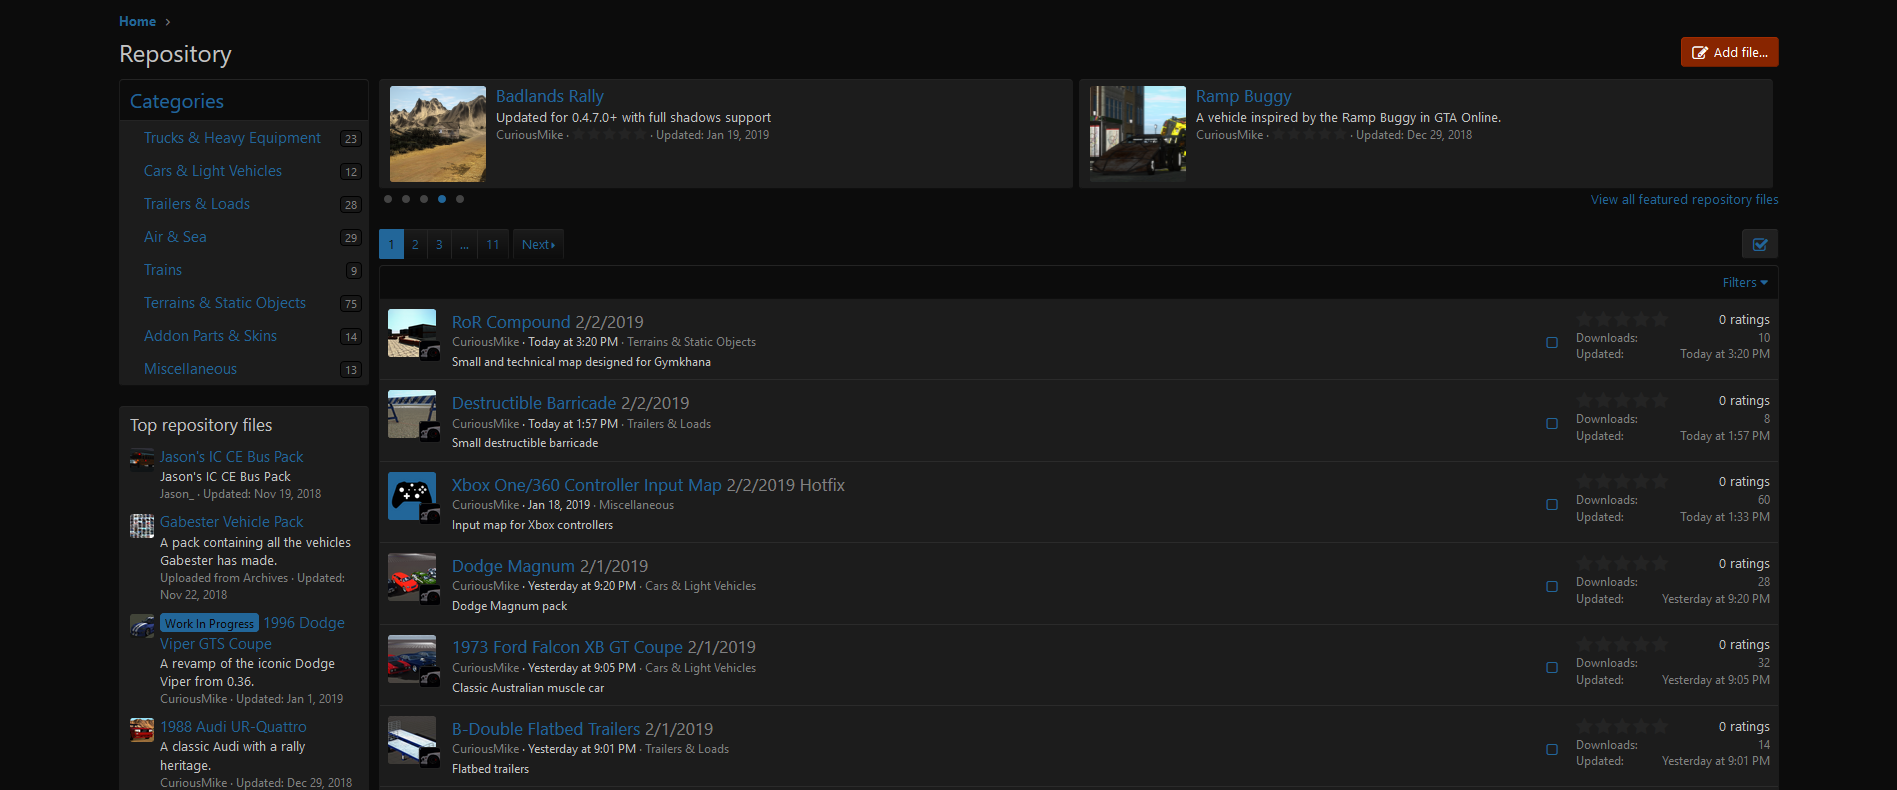
\includegraphics{images/repository.png}

Find something you like. For example, how about the nice
\href{https://forum.rigsofrods.org/resources/1996-dodge-viper-gts-coupe.88/}{1996
Dodge Viper GTS Coupe}:

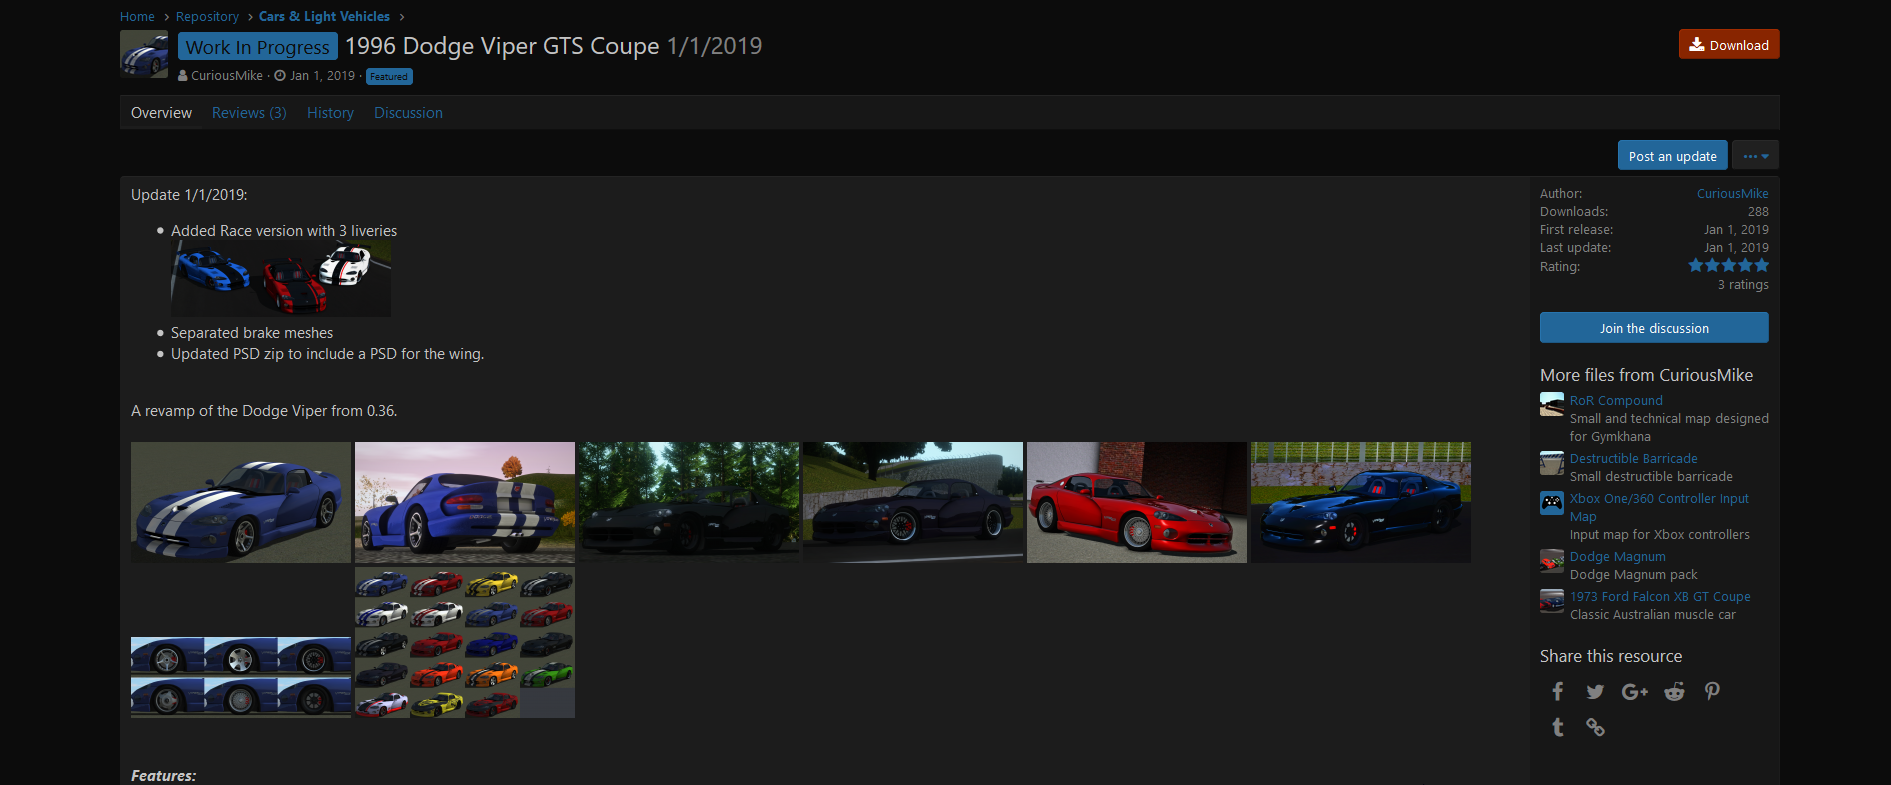
\includegraphics{images/repository-mod.png}

Click the \emph{Download} button at the top right of the page:


\includegraphics{images/repository-download.png}

\hypertarget{installing}{%
\subsection{Installing}\label{installing}}

Once the mod is downloaded, simply place the \texttt{*.zip} file into
\texttt{Documents\textbackslash{}Rigs\ of\ Rods\ 0.4\textbackslash{}mods}
or \texttt{\textasciitilde{}/.rigsofrods/mods} on Linux:

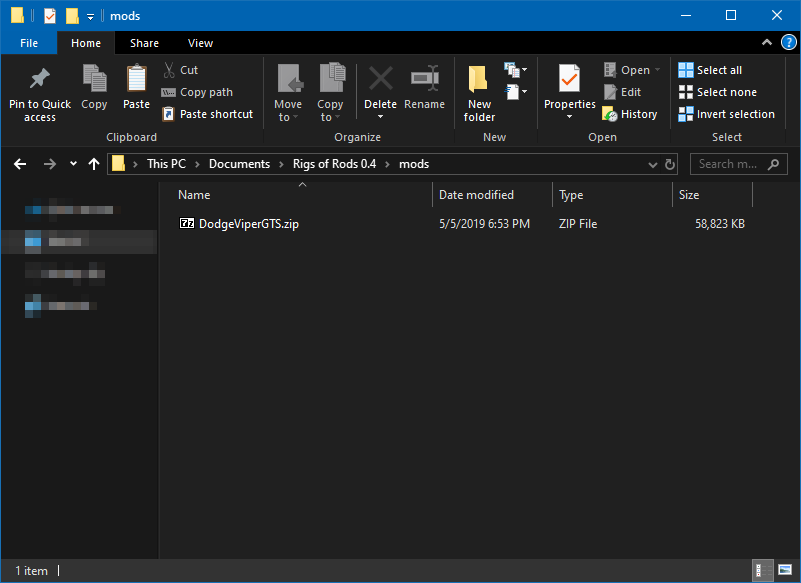
\includegraphics{images/repository-installing-mod.png}

\textbf{NEVER extract the zip file unless specifically mentioned in the
file description! I cannot stress this enough.}

You can organize your mods with subfolders.
(e.g.~\texttt{mods\textbackslash{}vehicles\textbackslash{}DodgeViperGTS.zip})

That's it! You can launch Rigs of Rods now and your shiny new mod should
be ready to use.

\hypertarget{installing-packs}{%
\section{Installing packs}\label{installing-packs}}

To install packs (a zip file containing multiple zips inside) such as
the
\href{http://forum.rigsofrods.org/resources/gabester-vehicle-pack.12/}{Gabester
Vehicle Pack} or the
\href{http://archives.rigsofrods.net/contentpacks/}{content packs}, just
extract the zip into the \texttt{mods} folder.

\hypertarget{installing-skinzips}{%
\section{Installing skinzips}\label{installing-skinzips}}

Some mods may provide a \texttt{*.skinzip} which contains some extra
liveries/skins for the vehicle. To install these, just place them inside
the \texttt{mods} folder.

For more information about skinzips, see
\href{/vehicle-creation/alternate-skins/}{this page}.

\hypertarget{psdpdn-files}{%
\section{PSD/PDN files}\label{psdpdn-files}}

These are files meant to be used by photo editing programs such as
Photoshop or paint.net, they are not meant to be placed in the RoR
directories.
